\part{Введение в практическую электронику}\label{collis}
\addcontentsline{toc}{section}{An Introduction to 
Practical Electronics, 
Microcontrollers and
Software Design \copyright\ Bill Collis}

Эта часть основана на книге:
\bigskip

\textbf{An Introduction to 
Practical Electronics, 
Microcontrollers and
Software Design}

Second Edition, 01 May-2014

\copyright\ Bill Collis

\url{www.techideas.co.nz}

\bigskip
Мы признательны автору за разрешение использовать материалы его книги в
русскоязычном варианте <<Азбуки>>, и конечно он вполне заслуженно включен в
основные соавторы этой книги.

\bigskip
We are grateful to the author for permission to use materials of his book in the
russian version of <<Azbuka>>, and of course he was deservedly included in the
main co-authors of this book.

\bigskip
\begin{verbatim}
From: Bill Collis <Bill.Collis@..........nz>
Date: 2014-11-24 0:53 GMT+04:00
Subject: Electronis Book
To: "dponyatov@gmail.com" <dponyatov@gmail.com>

Hi Dmitry
thanks for your email.
I am looking at the future of the book myself and thinking I will open source
it. If you will only be in using it in Russian language then that is ok and you
need to reference the original book.

Thanks
Bill
\end{verbatim}

\chapter{1 Введение в практическую электронику 13}

Эта книга\note{оригинал: B.Collis The Introduction to Practical 
Electronics\ldots}\ имеет слеующий ряд основных направлений:

\begin{itemize}
  \item Распознавание электронных компонентов и их правильное использование
  \item Наработка цельного набора компетенций в базовой электронике
  \item Использование макетных плат
  \item Навыки ручной пайки
  \item Использование закона Ома для выбора токоограничивающих резисторов
  \item Делитель напряжения
  \item Использование EDA CAD\note{\keys{E}\,lectronic \keys{D}\,esign
  \keys{A}\,utomation, САПР автоматизации проектирования электроники}\ для
  разработки и подготовки производства печатных плат
  \item Программирование микроконтроллеров и их сопряжение
  \item Транзистор в ключевом режиме
  \item Теория источников питания
  \item Принципы и схемы электропривода
  \item Моделирование решений через тестирование и испытания
  \item Следование кодексу практики
  \item Безопасные приемы работы
\end{itemize}

\section{Ваше обучение по специальности <<Технология>>}

\begin{itemize}

\item \textbf{Технологическая практика}

\begin{itemize}

\item\textbf{Быть четким}: разработка четких спецификаций для ваших
технологических проектов.

\item\textbf{Планирование}: думать прежде чем делать, и использовать во время
работы наброски типа блок-схем, принципиальных схем, чертежей разводки плат,
диаграмм и эскизов.

\item\textbf{Работа на результат}: испытания, тестирование и сборка электронных
схем, проектирование и изготовление печатных плат, написание программ для
микроконтроллеров.

\end{itemize}

\item \textbf{Технологические знания}

\begin{itemize}

\item\textbf{Технологическое моделирование}: прежде чем строить электронное
устройство, важно понять как оно работает сначала путем моделирования и/или
тестирования аппаратного и программного обеспечения.

\item\textbf{Технологические продукты}: знания о компонентах и ​​их
характеристиках.

\item\textbf{Технологические системы}: электронное устройство является более,
чем набором компонентов, это функционирующая система с входами, выходами и
контролирующим процессом.

\end{itemize}

\item \textbf{Nature of Technology}

\begin{itemize}

\item\textbf{Characteristics of Technological Outcomes} – knowing about
electronic components especially microcontrollers as the basis for modern technologies.

\item\textbf{Characteristics of Technology} – electronic devices now play a
central role in the infrastructure of our modern society; are we their masters, how have they changed our lives?

\end{itemize}

\end{itemize}

\section{Ключевые компетенции Ново-Зеландской программы}

\begin{itemize}

\item\textbf{Thinking} – to me the subject of technology is all about thinking.
My goal is to have students understand the technologies embedded within electronic devices. To achieve this students
must actively enage with their work at the earliest stage so that they can construct their own
understandings and go on to become good problem solvers. In the beginning of their learning
in electronics this requires students to make sense of the instructions they have been given
and search for clarity when they do not understand them. After that there are many new and
different pieces of knowledge introduced in class and students are given problem solving
exercises to help them think logically. The copying of someone elses answer is flawed but
working together is encouraged. At the core of learning isbuilding correct conceptual models
and to have things in the context of the ‘big picture’.

\item\textbf{Relating to others} – working together in pairs and groups is as
essential in the classroom as it is in any other situation in life; we all have to share and negotiate resources and equipment
with others; it is essential therefore to actively communicate with each other and assist one
other.

\item\textbf{Using language symbols and texts} – At the heart of our subject is
the language we use for communicating electronic circuits, concepts, algorithms and computer programming syntax; so
the ability to recognise and using symbols and diagrams correctly for the work we do is vital.

\item\textbf{Managing self} – This is about students taking personal
responsibility for their own learning; it is about challenging students who expect to read answers in a book or have a teacher tell them
what to do. It means that students need to engage with the material in front of them.
Sometimes the answers will come easily, sometimes they will not; often our subject involves a
lot of trial and error (mostly error). Students should know that it is in the tough times that the
most is learnt. And not to give up keep searching for understanding.

\item\textbf{Participating and contributing} – We live in a world that is
incredibly dependent upon technology especially electronics, students need to develop an awareness of the importance
of this area of human creativity to our daily lives and to recognise that our projects have a
social function as well as a technical one.

\end{itemize}


\secrel{Вводная электронная схема}\label{bcentry}\secdown

\secrel{Где купить комплектующие?}

В Новой Зеландии есть некоторое количество отличных поставщиков компонентов с
разумными ценами, включающих \url{www.surplustronics.co.nz}, и
\url{www.activecomponents.com}. Зарубежные поставщики, которых я использую,
включают \url{www.digikey.co.nz}, \url{www.sparkfun.com}, \url{ebay.com}
и \url{aliexpress.com}.

\bigskip
Для России можно отметить сеть магазинов
``\href{http://voltmaster.ru/}{Больтмастер}''\note{\href{http://voltmaster-samara.ru/}{Самара}}.

\bigskip
Для модулей пока что доступна поставка из Китая по почте:
\href{http://www.aliexpress.com/}{AliExpress}\ с оплатой с виртуальной карты
VISA платежной системы \href{https://qiwi.ru/}{QIWI}. Доставка занимает от 2х
недель до 2х месяцев. Удобно покупать модули в виде микросхем, уже запаянных с
обвязкой на кусок текстолита (\term{breakout board}): Arduino Mini, Maple Mini,
датчики, контроллеры двигателей. Также интересны наборы (магазины) элементов:
пачки резисторов, конденсаторов и т.п. в выводном исполнении, по нескольку
десятков номиналов.

\secrel{Макетная плата: \term{breadboard}}

\begin{youtube}
\url{https://www.youtube.com/watch?v=vQdUSE1auz8}

\url{https://www.youtube.com/watch?v=k9jcHB9tWko}

\url{https://www.youtube.com/watch?v=2wvn8_23phE}

\end{youtube}

\bigskip
\noindent
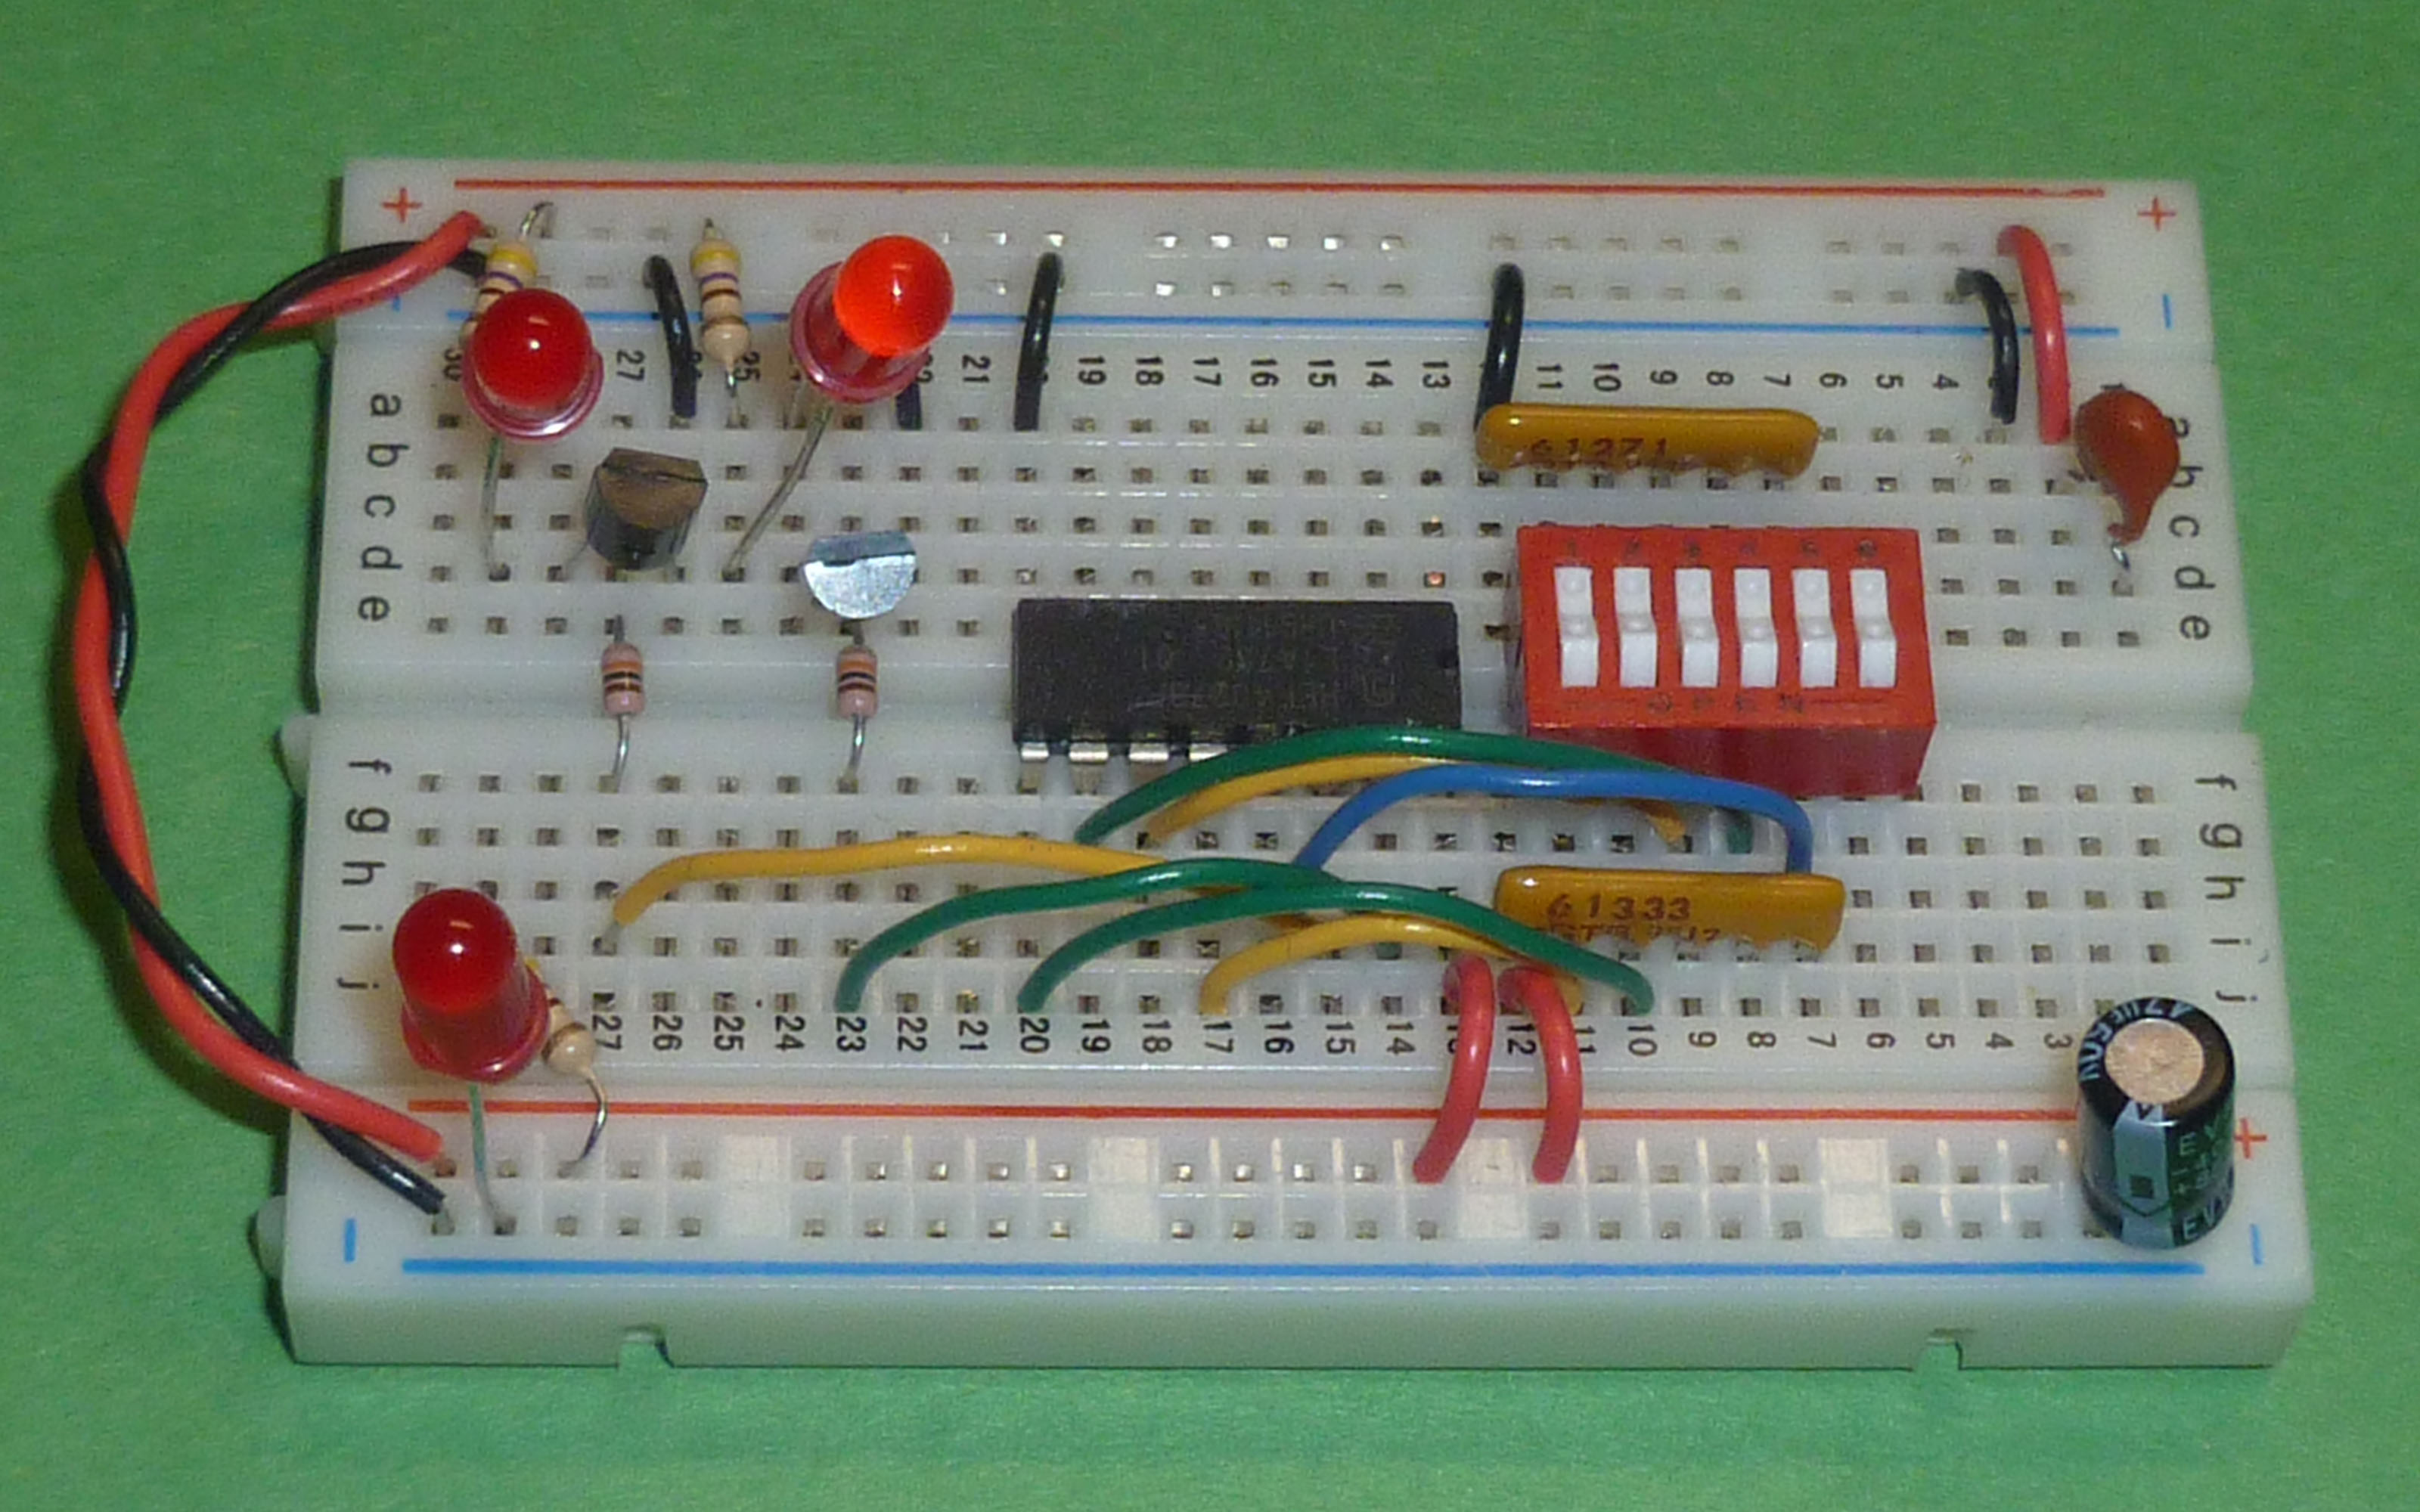
\includegraphics[height=0.3\textheight]{bcollis/breadboard2.jpg}
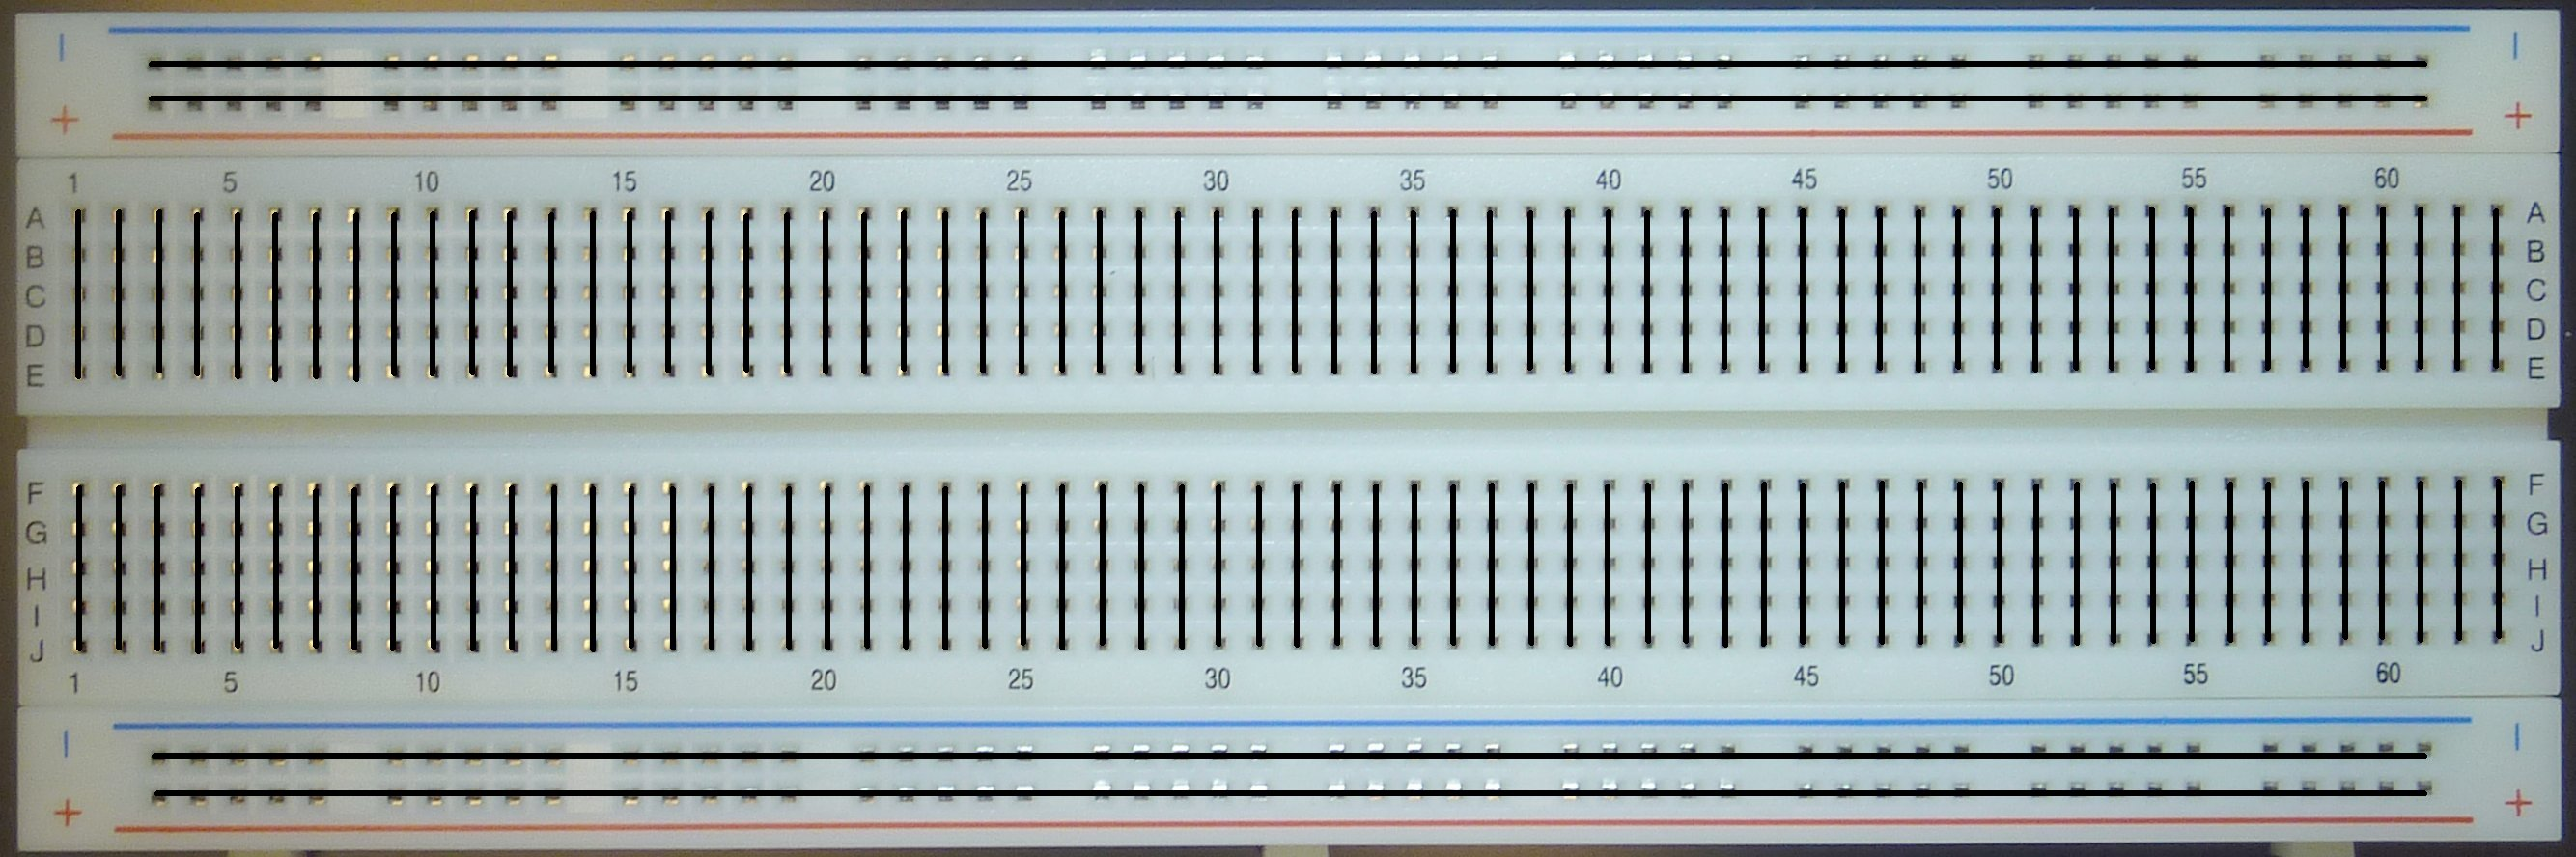
\includegraphics[height=0.3\textheight]{bcollis/BreadboardConnections.jpg}
\bigskip

\termdef{Breadboard}{breadboard} ([б]еспаечная \termdef{[м]акетная
[п]лата}{макетная плата} , \termdef{БМП}{БМП}, ``\termdef{вафля}{вафля}'')\ ---
пластмассовый блок с отверстиями и металлическими полоск\'{о}выми зажимами,
создающими соединения между \termdef{элементами схемы}{элемент}. Отверстия
расположены так, что \termdef{компоненты}{компонент} и отрезки провода могут
быть соединены вместе формируя схему, без использования паяльника. Верхние и
нижние ряды, как правило, используются для \termdef{шин питания}{шина питания},
красный сверху для плюса, и внизу черный/синий для минуса (\termdef{общий
провод}{общий провод}, или \termdef{``земля''}{земля}). На длинных вафлях шины
питания поделены на отдельные сегменты, и требуют соединения короткими
перемычками.

\secrel{Простейшая схема}

Эта схема может быть собрана вот так \ref{ch21lay}, обратите внимание, что
\termdef{светодиод}{светодиод} должен находиться в правильном положении. Если у
вас есть светодиод и \termdef{резистор}{резистор}, соединенные в
\termdef{замкнутый контур}{замкнутый контур}, светодиод должен загореться.

\bigskip
\noindent\begin{tabular}{p{0.45\textwidth} p{0.45\textwidth}}
Принципиальная схема \label{ch21sch}
&
Компоновка \label{ch21lay} \\
&\\
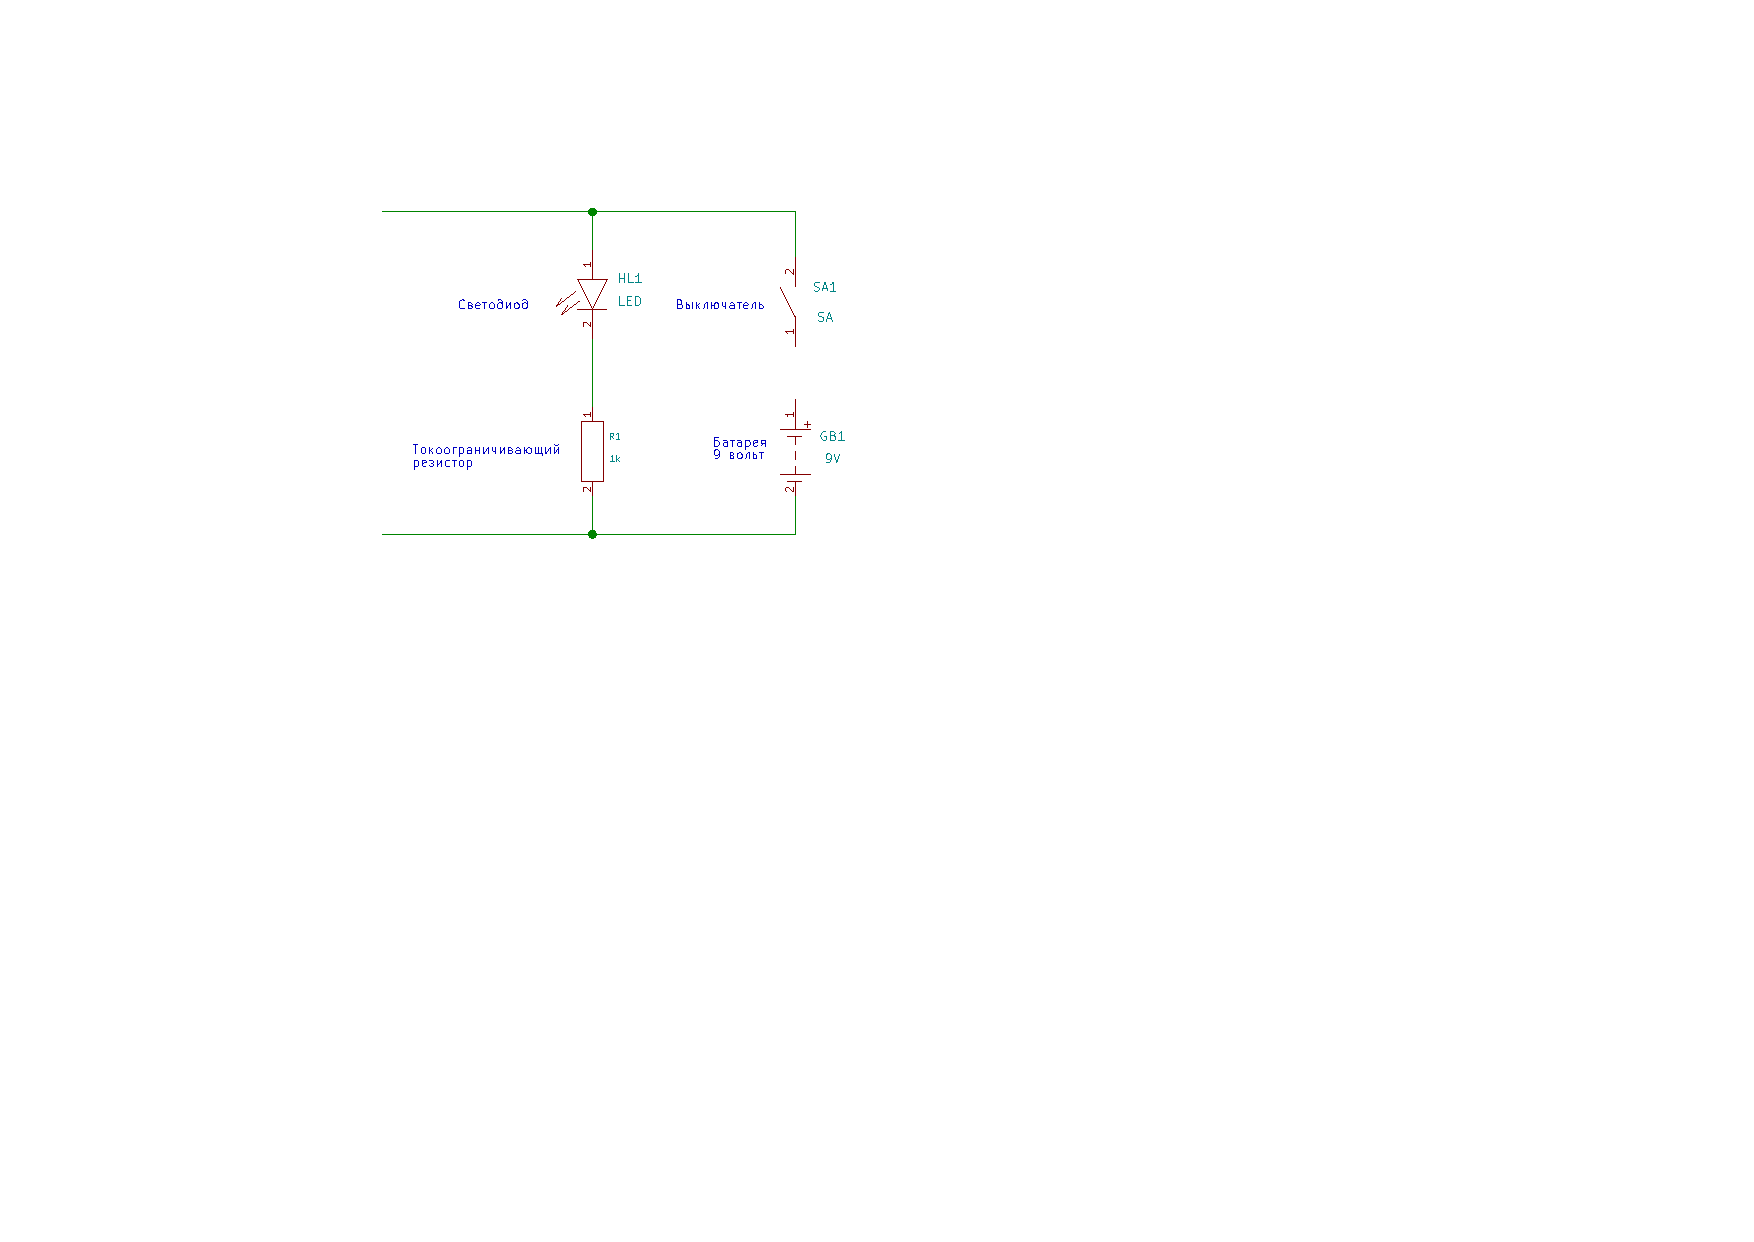
\includegraphics[width=0.45\textwidth]{bcollis/led1/led1.pdf}
&
\\
\end{tabular}

\bigskip
Светодиоду требуется \emph{для включения} около 2\,В\note{[В]ольт}, батарея на
9\,В, так что с напряжением все нормально. \emph{Но если вы подключите светодиод
напрямую к батарее, он сгорит! Для светодиодов главный рабочий параметр\ ---
\termdef{допустимый рабочий ток}{допустимый рабочий ток}, обычно он не превышает
10..20\,mA\note{1\,[м]иллиАмпер = 0.001\,[А]мпер}}. Так что
1\,k\note{1\,[К]илоОм = 1000\,Ом}\ резистор используется для ограничения тока
через светодиод.

\bigskip
Недопустимо подавать на светодиоды напряжение обратной полярности. Светодиоды
имеют невысокое (несколько вольт) обратное пробивное напряжение. В схемах, где
возможно появление обратного напряжения, светодиод должен быть защищён
параллельно включенным обычным диодом в противоположной полярности.

\bigskip
Если вы отключите любой провод в схеме, она перестает работать, схема должна
быть завершенной, чтобы электроны могли течь по проводникам из
\termdef{источника питания}{источник питания}.

\secrel{Ток и напряжение, сечение проводника, плотность тока}\label{bctok}

\begin{youtube}

\url{https://www.youtube.com/watch?v=Dq4fSp6wz-o}

\begin{enumerate}[nosep]
  \item \url{https://www.youtube.com/watch?v=3ZeveDL1\_bg}
  Электрический ток Источники тока
  \item \url{https://www.youtube.com/watch?v=mt86jYUjPFI}
  Ток в металлах Действия электрического тока 
  \item \url{https://www.youtube.com/watch?v=42CEi94hGgA}
  Электрический ток. Сила тока
  \item \url{https://www.youtube.com/watch?v=SNPO5e9wZWU}
  Амперметр Измерение силы тока
  \item \url{https://www.youtube.com/watch?v=Yt91alAwp68}
  Электрическое напряжение
\end{enumerate}

\end{youtube}

В предыдущем разделе были использованы два важных понятия электроники\ ---
\termdef{ток}{ток} и \termdef{напряжение}{напряжение}. Необходимо объяснить эти
понятия, не залезая глубоко в физику. Проще всего объяснить какое-то явление на
примере другого явления, с которым человек регуляроно сталкивается в обыденной
жизни, и ощущает его собственными органами чувств. Для электрических явлений
лучше всего подходит \termdef{гидравлическая модель}{гидравлическая
модель}\note{\href{http://edwpl.ucoz.ru/publ/fundamenty\_ehlektroniki/induktivnye_ehlementy/induktivnosti/5-1-0-18}{пример
применения} гидравлической модели, осторожно, г***осайт}.
В \termdef{ГМ}{ГМ} электрические явления заменяются условными водопроводными:
\termdef{проводник}{проводник}\ --- труба, \termdef{электрический
ток}{электрический ток}\ --- поток воды в этой трубе,
\termdef{резистор}{резистор}\ --- сужение сечения трубы, препятствующее течению
тока, \termdef{диод}{диод}\ --- клапан, открывающися только в одну сторону, и
т.п. В результате маловразумительные абстрактные понятия физики электрических
явлений превращаются в почти ощутимые потоки и давление воды: все мы ежедневно
пользуемся водопроводом, даже в глухих регионах найдется бочка или хотя
бы дырявое ведро.

\bigskip
Таким образом, любому школьнику можно объяснить эти понятия:

\begin{rulebox}
Электрическое \termdef{напряжение}{напряжение}\ --- давление ``электрической
воды'' в проводнике-трубе.\\
Измеряется в \termdef{[В]\'{о}льтах}{Вольт}. 
\end{rulebox}

Как и обычное давление, \emph{напряжение\ --- разностная величина, так как
измеряется между двумя точками} электрической цепи. Для обычного давления за
опорную величину принимают атмосферное давление\note{не ощущаемое человеком, так
как оно уравновешено таким же внутренним давлением крови}. Для электричества
напряжение измеряют тоже между двумя точками, или между точкой и \termdef{общим
проводом}{общий провод}, принимаемым за 0. В физике напряжение определяют также
как \termdef{разность потенциалов}{разность потенциалов} между двумя точками.

\begin{framed}\noindent
Если взять проводник, и разделить его условной плоскостью, перпендикулярной
проводнику, в области пересечения этой плоскости и проводника получается
область\ --- \termdef{сечение проводника}{сечение проводника}.
\end{framed}

Сечение проводника легко увидеть и реально\ --- достаточно взять
толстый одножильный сплошной провод, и аккуратно отпилить (не откусить) его
точно поперек. Поверхность такого отпила и будет сечением.

\begin{rulebox}
Электрический \termdef{ток}{ток}\ --- количество ``электрической
воды'', проходящей через сечение проводника-трубы в единицу времени.
\termdef{Сила тока}{сила тока} измеряется в \termdef{[А]мп\'{е}рах}{Ампер}.
\end{rulebox}

\begin{framed}\noindent
\begin{equation}
j = \frac{I}{S}
\end{equation}
\begin{tabular}{l l l}
где& $j$ & \termdef{плотность тока}{плотность тока}, $\mbox{А}/\mbox{м}^{2}$ \\
&$I$ & сила тока, Ампер \\
&$S$ & \termdef{площадь сечения проводника}{площадь сечения проводника},
$\mbox{м}^{2}$
\end{tabular}
\end{framed}

Чем выше плотность тока, тем больше нагревается проводник (подробнее см
\ref{joul}), поэтому она учитывается при выборе провода, и ширины приводников
печатных плат. В этом случае часто используется численно другая величина\ ---
$\mbox{А}/\mbox{мм}^{2}$.

\secrel{Проводники и изоляторы, сопротивление и проводимость}\label{bcohm}

\begin{youtube}
\begin{enumerate}[nosep]
  \item \url{https://www.youtube.com/watch?v=q4I1hZ5YQ2w}
Электрическое сопротивление проводника.    
  \item \url{https://www.youtube.com/watch?v=SlxOEEaQ4Cg}
Удельное сопротивление 
\end{enumerate}

\url{https://www.youtube.com/watch?v=FCkR-3YE5Ac}

\end{youtube}

Используя гидравлическую модель, точно так же просто можно объяснить понятие
\termdef{проводимости}{проводимость}. Любой материал можно представить как
кусок вещества, имеющий пористую структуру, например как поролон или песок.
Через этот пористый материал течет ``электрическая вода'', т.е. ток. Это течение
вызвано действием напряжения, \term{приложенного} к концам проводника
(источником питания). Напряжение проталкивает электричество через материал,
поэтому чем больше напряжение, тем выше сила проходящего тока. Каждый материал
имееет свою ``пористость'', чем она больше, тем больше \term{проводимость}:

\begin{framed}
\begin{equation}\label{igu}
I = G \ U
\end{equation}
\begin{tabular}{l l l}
где & $I$ & сила тока, А \\
& $G$ & проводимость, См (сименс) \\
& $U$ & напряжение, В \\ 
\end{tabular}
\end{framed}

Чаще вместо проводимости используют обратную величину\ ---
\termdef{сопротивление}{сопротивление}:

\begin{framed}
\begin{equation}
R = \frac{1}{G} = G^{-1}
\end{equation}
\begin{tabular}{l l l}
где & $G$ & проводимость, См (сименс)\\
& $R$ & сопротивление, Ом\\
\end{tabular}
\end{framed}

Соответственно, формула \ref{igu}\ превращается в описанный в любом школьном
учебнике физики \termdef{закон Ома для постоянного тока}{закон Ома!для
постоянного тока}:

\begin{rulebox}
\begin{equation}\label{ohmlaw}
I = \frac{R}{U}
\end{equation}
\end{rulebox}

В зависимости от проводимости или сопротивления материалы делят на несколько
видов:

\bigskip
\begin{tabular}{ l l l }
& $G$, проводимость & $R$, сопротивление \\
\hline
сверхпроводник & $\infty$ & 0 \\ 
\termdef{проводник}{проводник} & большая & низкое \\
\termdef{изолятор}{изолятор}, 
\termdef{диэлектрик}{диэлектрик} & низкая & высокое \\
\end{tabular}
\bigskip

В зависимости от внешних условий: температуры, давления, агрегатного состояния
вещества\note{плазма, газ, жидкость, твердое тело}, примесей\ --- одно и то же
вещество может быть как проводником, так и изолятором.

Типичные проводники: металлы, ионизированный газ (плазма), растворы солей в воде
(электролиты), \emph{влажное} дерево

Типичные диэлектрики: пластики, стекло, керамика, \emph{сухое} дерево, вакуум,
газы в т.ч. воздух.

\bigskip
В электронике очень часто нужно иметь в определенном месте схемы заданное
сопротивление, для этого выпускаются специальные элементы с \emph{точно
калиброванным сопротивлением} между \termdef{выводами}{вывод элемента}:
\termdef{резисторы}{резистор}, иногда применяют устаревшее название \termdef{сопротивление}{сопротивление}
(часто проволочное). Их делают из керамики, на которую наматывают проволоку, или
напыляют тонкую пленку из специальных металлических сплавов с высоким
сопротивлением\note{часто в состав входят никель, хром, вольфрам}.
Иногда используется только кусочек такого сплава без керамики.
Для качественной пайки выводы резисторов делают из хорошо проводящего металла,
хорошо смачиваемого расплавленным припоем.

\secrel{Диэлектрическая и тепловая прочность изоляции}\label{bcisol}

\bigskip
Для диэлектриков существует специальный параметр, характеризующий их способность
работать как изолятор\ --- \termdef{диэлектрическая прочность}{диэлектрическая
прочность}.

\begin{framed}\noindent
Чем выше диэлектрическая прочность, тем большее напряжение способен выдерживать
изолятор без разрушения.
\end{framed}

\begin{framed}\noindent
При повышении температуры диэлектрическая прочность уменьшается 
\end{framed}

Именно поэтому

\begin{alarmbox}
Запрещается использовать любые удлинители в свернутом состоянии, или
использовать электрический провод, свернутый бухтой (катушкой)
\end{alarmbox}

\begin{alarmbox}
Не допускается нагрев любых частей электронной схемы или элементов
конструкции выше 40..50$^{o}C$
\end{alarmbox}

Для любого диалектрика существует некоторое значение напряжения, при котором он
начинает пропускать ток. При прохождении тока материал нагревается (\ref{joul}).
В результате нагрева проходящим током или от соседних соприкасающихся
поверхностей у диэлектрика увеличивается проводимость, что приводит к еще
большему проходящему через него току, и дополнительному нагреву. 

Если тепло не отводится во внешнюю среду (например в середине катушки провода
смотанного удлинителя), температура продолжает повышаться. В некоторый момент
температура достигает значения, при котором слой изоляции размягчается,
утрачивает механическую прочность, и соседние проводники сближаются или
соприкасаются с плохим контактом (происходит \termdef{короткое
замыкание}{короткое замыкание}).

\alarm{В месте плохого контакта или большого тока температура резко повышается}
до значений, когда диалектрик воспламеняется или резко меняет химический состав,
распадаясь \emph{с выделением ядовитых соединений}\note{для типичной изоляции из
ПВХ\ --- сложные токсичные соединения с содержанием хлора} и полностью утрачивая
изолирующие свойства как в электрическом, так и в механическом смысле.

Самый опасный вариант, и типичный случай \termdef{выгорания проводки}{выгорание
проводки}\ --- \termdef{ток короткого замыкания}{ток короткого замыкания}
слишком маленький для срабатывания защитных устройств
(\termdef{предохранитель}{предохранитель}, \termdef{автомат}{автомат},
\termdef{устройство защитного отключения}{устройство защитного
отключения}, \termdef{УЗО}{УЗО}), но достаточный для нагрева изоляции до
температуры химического распада или воспламенения. Аварийного выключения не
происходит, а проводка продолжает гореть до победного конца. 

\secrel{Тепловое действие тока. Мощность}

\begin{youtube}
\begin{enumerate}[nosep]
  \item \url{https://www.youtube.com/watch?v=2LWAIOHRI8s}
  Нагревание проводников электрическим током \termdef{Закон Джоуля Ленца}{закон
  Джоуля Ленца}
  \item \url{https://www.youtube.com/watch?v=Mbt4OTgBRuw}
  \termdef{Мощность}{мощность} электрического тока
\end{enumerate}
\end{youtube}

\secrel{Масштабные множители}\label{bcmux}

\begin{youtube}
\url{https://www.youtube.com/watch?v=i3ABWmCl1EI} Перевод единиц измерения
\end{youtube}

Практически для всех единиц измерения необходимо использование
\termdef{масштабных множителей}{масштабные множители}, когда величины численно
или слишком большие (много цифр до запятой), или слишком маленькие (много цифр
после запятой):

\bigskip
\begin{tabular}{ l l l }
пико & p & $10^{-12}$ \\
nano & n & $10^{-9}$ \\ 
микро & u, $\mu$ & $10^{-6}$ \\ 
милли & m & $10^{-3}$ \\
\hline
кило & k, K & $10^{3}$ \\
мега & M & $10^{6}$ \\
гига & G & $10^{9}$ \\
\end{tabular}
\bigskip

10\,mA = $10 \times 10^{-3}$\ A = $10 \times 0.001$ A = 0.010 A

5\,КОм = $5 \times 10^{3}$ Ом = $5 \times 1000$ Ом = 5000 Ом

\secrel{Использование мультиметра}\label{bcmmetr}

\begin{youtube}
\url{https://www.youtube.com/watch?v=BEgvm4o-u2Q}

\url{https://www.youtube.com/watch?v=UMwYLwsPgCY}

\begin{enumerate}[nosep]
  \item \url{https://www.youtube.com/watch?v=GBuGSj1uPGk}
  \item \url{https://www.youtube.com/watch?v=VJ3RBS42IVY}
\end{enumerate}

\url{https://www.youtube.com/watch?v=q3R4s6WE1cI}
\end{youtube}

Возьмите мультиметр (\ref{mmetr}) и измерьте напряжение на резисторе, близко ли
оно к 7\,В ? Также измерьте ток через диод, не превышает ли он допустимый ?

\begin{framed}
\emph{Напряжение} измеряется \term{в [В]\'{о}льтах} подключением
\term{измерительного прибора} (мультиметра) \emph{параллельно}\ элементу, при этом нужно
\begin{itemize}
\item
\term{режим измерения} включить на
\term{режим измерения постоянного напряжение} $V-$/DCV (или переменного,
обозначается как $V\sim$/ACV) а
  \item \term{диапазон
измерения} \emph{выставить на максимальное значение напряжения}
\item
Последовательно уменьшая диапазон измерения, найдите диапазон, в котором
мультиметр показывает наибольшее количество знаков после запятой.
\end{itemize}
\end{framed}

Если диапазон
слишком большой, прибор покажет значение в районе 0, а если слишком низкий\ ---
выведет [1]. Обычно работают в диапазоне, соответствующем максимальому
напряжению питания (в нашем случае 20\,V\note{[V]olt = [В]ольт}), иногда для
слабых напряжений переключаясь на одну..две ступени ниже. Но\ ---
\emph{возможны случаи\note{в \emph{любых схемах} содержащих
\term{индуктивности}: катушки пр\'{о}вода, трансформаторы, электродвигатели,
динамики и т.п.} когда напряжение в части схемы на порядки (в десятки..тысячи
раз) превосходит напряжение питания}.

\begin{framed}
\emph{Ток} измеряется \term{в [А]мп\'{е}рах} подключением \term{измерительного
прибора} (мультиметра) \emph{последовательно}\ с элементом \term{в разрыв цепи}, при этом
нужно
\begin{itemize}
\item
\term{режим измерения} включить на
\term{режим измерения постоянного тока} $A-$/DCA (или переменного, обозначается
как $A\sim$/ACA) а
  \item \term{диапазон
измерения} \emph{выставить на максимальное значение тока}
\item
Последовательно уменьшая диапазон измерения, найдите диапазон, в котором
мультиметр показывает наибольшее количество знаков после запятой.
\end{itemize}
\end{framed}

Обратите внимание, что напряжение измеряется \term{вольтметром} на полностью
собранной схеме, а для измерения тока нужно изменять схему, включая в нее
\term{амперметр}. Если измерения тока нужно проводить на готовом устройстве,
иногда ставят 2хконтактный \term{джампер} (как на материнских платах
компьютеров): при измерении амперметр подключают к его контактам, а потом
джампер замыкают специальной съемной проводящей перемычкой. Этом прием вы можете
использовать в своих устройствах для регулярного измерения \term{тока
потребления}, и расчета \term{потребляемой мощности}:

\begin{equation}
W_{\mbox{потребляемая}}\mbox{[Ватт]} =
U_{\mbox{питания}}\mbox{[Вольт]}
\times
I_{\mbox{устройства/элемента}}\mbox{[Ампер]}
\end{equation}

\begin{framed}
Переключив мультиметр в \term{режим прозвонки (т\'{е}стера)}, можно проверить
\begin{itemize}
\item наличие
электрического соединения между двумя точками \emph{обязательно отключенной от
источника питания} схемы,
\item исправность диода или светодиода,
\item исправность конденсатора большой \term{емкости} и
\item любые другие случаи когда нужно определить что две точки электрически
соединены между собой, постоянно или временно.
\end{itemize}
\end{framed}

Если между \term{щщуп}ами мультиметра в режиме прозвонки\note{= тестера}\
\term{сопротивление} протекающему току не превышает 1\,КилоОм\note{см.
паспорт на прибор}, раздается звуковой сигнал.

Если щщупы подключить к исправному \emph{разряженному} конденсатору большой
емкости (``электролиту''), раздастся короткий целчок или даже ``пик''.

Тестером также можно определить тип и \term{цокол\'{е}вку\note{``раскопытку''}}
транзистора; как это сделать описано в \ref{vt}.

\emph{Диоды} проверяются двумя подключениями \emph{в разной полярности}\ --- при
\emph{красном щщупе} на \term{аноде (+)} диода (в \term{прямой полярности
включения}) диод проводит ток, а в \term{обратной полярности} нет (красный щщуп
на \term{катоде (-)}).

Проверьте \emph{светодиод}: отключите его из схемы, и проверьте как диод.
Если светодиод исправен, в \emph{прямой полярности} светодиод будет \emph{очень
слабо светиться}.

\secrel{Определение сопротивления резистора по цветовому коду}

Когда берете резистор, проверьте его \termdef{номинал}{номинал} (значение). В
наших схемах каждый резистор имеет свою цель, и значение выбирается в
зависимости от того, хотим ли мы б\'{о}льший или меньший ток в этой части цепи.
Чем выше \term{номинал} резистора, тем меньше ток. Чем ниже номинал резистора,
тем выше ток. Для \termdef{выводн\'{ы}х}{выводн\'{о}й корпус} резисторов,
которые мы будем использовать на макетках, маркировка наносится на корпус в
виде набора цветных полосок:

\bigskip
Цветовая маркировка на 5 цветных полосок:
\begin{tabular}{|l|l|l|l|l|}
\hline
 цифра & цифра & цифра & множитель & точность \\
\hline
\end{tabular}

\bigskip Цифра:
\begin{tabular}{l l l l l l l l l l}
0&1&2&3&4&5&6&7&8&9\\
\textcolor{Black}{$\blacksquare$} &
\textcolor{Brown}{$\blacksquare$} &
\textcolor{Red}{$\blacksquare$} &
\textcolor{Orange}{$\blacksquare$} &
\textcolor{Yellow}{$\blacksquare$} &
\textcolor{Green}{$\blacksquare$} &
\textcolor{Blue}{$\blacksquare$} &
\textcolor{Magenta}{$\blacksquare$} &
\textcolor{Grey}{$\blacksquare$} &
$\square$ \\
\end{tabular}

\bigskip Множитель:
\begin{tabular}{l l l l l l l l l l}
\textcolor{Black}{$\blacksquare$} & $10^{0}=1$ &
\textcolor{Brown}{$\blacksquare$} & $10^{1}=10$ &
\textcolor{Red}{$\blacksquare$} & $10^{2}=100$ &
\textcolor{Orange}{$\blacksquare$} & $10^{3}=1000$ \\
\textcolor{Yellow}{$\blacksquare$} & $10^{4}=10000$ &
\textcolor{Green}{$\blacksquare$} & $10^{5}=100000$ &
\textcolor{Blue}{$\blacksquare$} & $10^{6}=1000000$ \\
\textcolor{Gold}{$\blacksquare$} & $10^{-1}=0.1$ &
\textcolor{Silver}{$\blacksquare$} & $10^{-2}=0.01$ \\
\end{tabular}

\bigskip Точность:
\begin{tabular}{l l l l l l l l l l l}
\textcolor{Brown}{$\blacksquare$} & $\pm 1\%$ &
\textcolor{Red}{$\blacksquare$} & $\pm 2\%$ &
\textcolor{Gold}{$\blacksquare$} & $\pm 5\%$ &
\textcolor{Silver}{$\blacksquare$} & $\pm 10\%$ \\
\end{tabular}

\bigskip
\begin{tabular}{l l l l l l l l l l l l l}
-[&
\textcolor{Brown}{$\blacksquare$}&
\textcolor{Black}{$\blacksquare$}&
\textcolor{Black}{$\blacksquare$}&
\textcolor{Yellow}{$\blacksquare$}&
\textcolor{Brown}{$\blacksquare$}&
]- 
& $100\times 10^{4}\pm 1\%$ & 1M & 1 миллион Ом & 1M $\Omega$ & 1 000 000 Ом \\
&1&0&0&4&1\\
-[&
\textcolor{Brown}{$\blacksquare$}&
\textcolor{Black}{$\blacksquare$}&
\textcolor{Black}{$\blacksquare$}&
\textcolor{Red}{$\blacksquare$}&
\textcolor{Red}{$\blacksquare$}&
]- 
& $100\times 10^{2}\pm 2\%$ & 10k & 10 тысяч ом & 10,000 Ом & 10k $\Omega$ \\
&1&0&0&2&2\\
-[&
\textcolor{Brown}{$\blacksquare$}&
\textcolor{Black}{$\blacksquare$}&
\textcolor{Black}{$\blacksquare$}&
\textcolor{Brown}{$\blacksquare$}&
\textcolor{Gold}{$\blacksquare$}&
]- 
& $100\times 10^{1}\pm 5\%$ & 1k & 1 тысяча ом & 1000 Ом & 1k $\Omega$ \\
&1&0&0&1&5\\
-[&
\textcolor{Orange}{$\blacksquare$}&
$\square$&
$\blacksquare$&
\textcolor{Black}{$\blacksquare$}&
\textcolor{Brown}{$\blacksquare$}&
]- 
& $390\times 10^{0}\pm 1\%$ & 390R & 390 Ом & 390$\Omega$ \\
&3&9&0&0&1\\
-[&
\textcolor{Brown}{$\blacksquare$}&
\textcolor{Black}{$\blacksquare$}&
\textcolor{Black}{$\blacksquare$}&
\textcolor{Black}{$\blacksquare$}&
\textcolor{Brown}{$\blacksquare$}&
]- 
& $100\times 10^{0}\pm 1\%$ & 100R & 1000 Ом & 100$\Omega$ \\
&1&0&0&0&1\\
-[&
\textcolor{Yellow}{$\blacksquare$}&
\textcolor{Magenta}{$\blacksquare$}&
\textcolor{Black}{$\blacksquare$}&
\textcolor{Gold}{$\blacksquare$}&
\textcolor{Brown}{$\blacksquare$}&
]- 
& $470\times 10^{-1}\pm 1\%$ & 47R & 47 Ом & 47$\Omega$ \\
&4&7&0&-1&1\\
\end{tabular}

\secrel{Светодиоды}

\noindent
\begin{tabular}{p{0.7\textwidth}p{0.3\textwidth}}
\noindent\parbox[b]{0.65\textwidth}{В настоящее время светоизлучающие диоды
используются в индикаторах и дисплеях на различном оборудовании, однако они все
больше и больше используются в качестве замены для \termdef{галогенных
ламп}{лампа!галогенная} и \termdef{ламп
накаливания}{лампа!накаливания}\note{использующие светящиеся проводники внутри
стеклянных колб} во многих других приложениях. Они включают в себя ходовые огни
на транспорте, светофоры,  большие уличные TV-экраны.}&
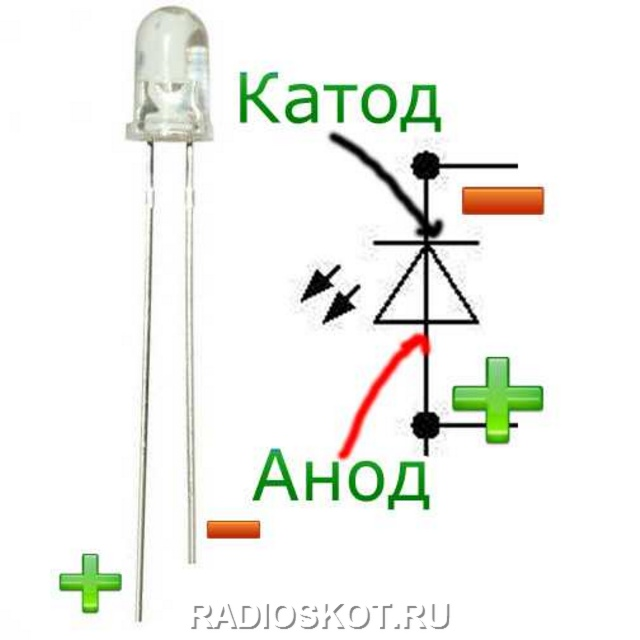
\includegraphics[width=0.25\textwidth]{bcollis/led.jpeg}
\\
\end{tabular}

\noindent
\begin{tabular}{p{0.3\textwidth} p{0.7\textwidth}}
\noindent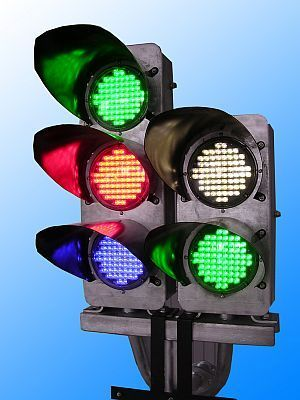
\includegraphics[width=0.3\textwidth]{bcollis/ledtraffic.jpeg}&
\noindent\parbox[b]{0.65\textwidth}{По сравнению с \term{лампами накаливания},
светодиоды почти не дают тепла, и поэтому очень эффективны. Они также имеют
гораздо б\'{о}льшее время жизни, например 10 лет, по сравнению с 10 месяцами для
ламп накаливания. Таким образом, в некоторых ситуациях например сигналов
светофора, если там установлены светодиоды, они дают значительную экономию как
по потребляемой мощности, так и по стоимости технического обслуживания. Хотя
есть небольшая проблема со светодиодными светофорами\ --- они не плавят снег,
который на них налипает!}\\
\end{tabular}

\secrel{Некоторые характеристики светодиодов}

\paragraph{\termdef{Интенсивность}{интенсивность}}: измеряется в мКд
(милликанделлах)

\paragraph{\termdef{Угол обзора}{угол обзора}}: угол от оси, до линии, где
интенсивность падает до 50\%

\paragraph{\termdef{Прямое напряжение}{прямое напряжение!светодиода}}:
напряжение необходимое для получения полной яркости светодиода

\paragraph{\termdef{Прямой ток}{прямой ток!светодиода}}: рабочий ток, дающий
максимальную яркость

\paragraph{\termdef{Пиковая длина волны}{пиковая длина волны}}: самая яркая
спектральная линия излучаемого света

\secrel{Задание на исследование светодиода}

Пользуясь сайтом одного из поставщиков, найдите информацию и
характеристики/атрибуты для двух светодиодов: обычный красный 5 мм и 5 мм
высокой интенсивности.


\bigskip
\begin{tabular}{|l|p{0.3\textwidth}|p{0.3\textwidth}|}

Cветодиод
&
Красный 5\,мм
&
Высокая интенсивность 5\,мм
\\
\hline

Поставщик&&\\

Номер детали&&\\

Стоимость (\$)&&\\

Яркость (мКд)&&\\

Прямое напряжение ($U_{F}$)&&\\

Длина волны (нм)&&\\

Прямой ток ($I_{F}$)&&\\

\end{tabular}

\clearpage\secrel{Добавление выключателя в схему}

Выключатель\ --- способ для ручного управления схемой пользователем

\bigskip\noindent
\begin{tabular}{p{0.45\textwidth} p{0.45\textwidth}}
Принципиальная схема
&
Компоновка
\\
\noindent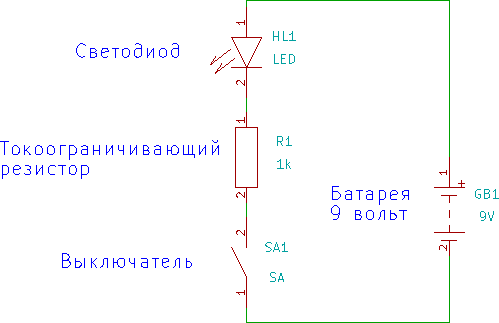
\includegraphics[width=0.45\textwidth]{bcollis/led2/led2.pdf}
&
\\
\end{tabular}

\secrel{2.7 Задание на установку выключателя 18}

2.7 Switch assignment

Find a small switch and carefully disassemble it (take it apart) draw how it
works and explain its operation. Make sure you explain the purpose of the
spring(s).

Here are simplified drawings of a small slide switch when it is in both
positions. When the switch is on electricity can flow, when it is open the
circuit is broken.


\secrel{Важные понятия схемотехники}

Кратко повторим:
\bigskip

Схема состоит из нескольких компонентов и источника питания, соединенных
проводами.

\emph{Поток электронов} (часто называют \termdef{носители заряда}{носители
заряда}) течет в цепи; однако если нет \emph{полной (замкнутой) цепи}, электроны
не могут течь.

\emph{Напряжение} (U) является мерой энергии в цепи, оно используется в качестве
меры энергии, подаваемой от батареи или энергии (напряжения) через часть схемы.

\emph{Ток (I) представляет собой поток электронов} от батареи по контуру и
обратно к батарее. Ток измеряется в амперах (обычно мы будем использовать
миллиампер или мА). Обратите внимание, что \emph{электрический ток это не ток
электронов или ток зарядов}. Так же, как течение реки не эквивалентно потоку
воды.

\emph{Сопротивление} работает \emph{на уменьшение тока}, резисторы в схеме
оказывают сопротивление току.

\emph{Проводники}, такие как провода, соединяющие компоненты вместе, не имеют
(теоретически) никакого сопротивления току.

\bigskip
Действительно важное понятие, для ясного понимания:

Напряжение прикладывается параллельно компонентам, а ток течет через компоненты.


% % \secrel{2.9 Изменение величины сопротивления 19}
% % \secrel{2.10 Добавление транзистора в схему 20}
% % \secrel{2.11 Чтение схем 21}
% % \secrel{2.12 Входная цепь\ --- LDR 22}
% % \secrel{2.13 Рабочая схема датчика темноты 23}
% % \secrel{2,14 Защитные цепи - использование диода 24}
% % \secrel{2.15 Задача исследования диода 24}
% % \secrel{2.13 Финальная схема датчика темноты 23}

\secup


\chapter{3 Вводное конструирование печатной платы 26}
% 3.1 Eagle Schematic and Layout Editor Tutorial  26
% 3.2 An Introduction to Eagle  27
% 3.3 The Schematic Editor  28
% 3.4 The Board Editor . 33
% 3.5 Making Negative Printouts . 37
% 3.6 PCB Making  38
\chapter{4 Пайка, припой и паяльники 41}
% 4.1 Soldering facts . 42
% 4.2 Soldering Safety  42
% 4.3 Soldering wires to switches  43
% 4.4 Codes of practice  44
% 4.5 Good and bad solder joints  45
% 4.6 Short circuits . 46
% 4.7 Soldering wires to LED’s . 48
\chapter{5 Введение в теорию электроники 49}
% 5.1 Making electricity  49
% 5.2 ESD electrostatic discharge  51
% 5.3 Magnets, wires and motion  52
% 5.4 Group Power Assignment  52
% 5.5 Electricity supply in New Zealand  53
% 5.6 Conductors  54
% 5.7 Insulators  54
% 5.8 Choosing the right wire  55
% 5.9 Resistors . 56
% 5.10 Resistor Assignment . 56
% 5.11 Resistivity  56
% 5.12 Resistor prefixes . 57
% 5.13 Resistor Values Exercises . 58
% 5.14 Capacitors  60
% 5.15 Component symbols reference  61
% 5.16 Year 10/11 - Typical test questions so far  62
\chapter{6 Введение в электронику микроконтроллера 63}
% 6.1 What is a computer? . 64
% 6.2 What does a computer system do?  64
% 6.3 What does a microcontroller system do? . 65
% 6.4 What exactly is a microcontroller?  66
% 6.5 Getting started with AVR Programming  67
% 6.6 Breadboard  67
% 6.7 Breadboard+Prototyping board circuit  68
% 6.8 Checking your workmanship . 70
% 6.9 Getting started with Bascom & AVR  71
% 6.10 The compiler . 71
% 6.11 The programmer . 71
% 6.12 USBASP programming cable  72
% 6.13 Your first circuit  73
% 6.14 An introduction to flowcharts . 74
% 6.15 Bascom output commands . 75
% 6.16 Exercises  76
% 6.17 Two delays . 77
% 6.18 Syntax errors -‘bugs’ . 78
% 6.19 Microcontroller portswrite a Knightrider program using LED’s  79
% 6.20 Knightrider v2  80
% 6.21 Knightrider v3  81
% 6.22 Commenting your programs  83
% 6.23 Learning review  83
% 6.24 What is a piezo and how does it make sound?. 84
% 6.25 Sounding Off . 85
% 6.26 Sound exercises . 87
% 6.27 Amp it up . 88
\chapter{7 Входные цепи микроконтроллера 91}
% 7.1 Single push button switch  91
% 7.2 Pullup resistor theory  93
% 7.3 Switch in a breadboard circuit  93
% 7.4 Checking switches in your program  94
% 7.5 Program Logic – the ‘If-Then’ Switch Test  95
% 7.6 If-then exercises  96
% 7.7 Switch contact bounce . 97
% 7.8 Reading multiple switches  99
% 7.9 Bascom debounce command . 100
% 7.10 Different types of switches you can use  101
% 7.11 Reflective opto switch  102
\chapter{8 Обзор программирования 104}
% 8.1 Three steps to help you write good programs  104
% 8.2 Saving Programs . 104
% 8.3 Organisation is everything  104
% 8.4 Programming template  105
% 8.5 What you do when learning to program . 106
% 8.6 AVR microcontroller hardware  107
% 8.7 Power supplies 107
% 8.8 Programming words you need to be able to use correctly  110
% 8.9 Year10/11 typical test questions so far  111
\chapter{9 Введение в поток выполнения программы 112}
% 9.1 Pedestrian crossing lights controller  112
% 9.2 Pedestrian Crossing Lights schematic  113
% 9.3 Pedestrian Crossing Lights PCB Layout 114
% 9.4 Algorithm planning example – pedestrian crossing lights . 115
% 9.5 Flowchart planning example – pedestrian crossing lights . 116
% 9.6 Getting started code  117
% 9.7 Modification exercise for the pedestrian crossing . 117
% 9.8 Traffic lights program flow  118
\chapter{10 Вводное программирование: использование подпрограмм 126}
% 10.1 Sending Morse code  127
% 10.2 LM386 audio amplifier PCB. 130
% 10.3 LM386 PCB Layout . 132
\chapter{11 Вводное программирование: Использование переменных 134}
% 11.1 Stepping or counting using variables  135
% 11.2 For-Next  137
% 11.3 Siren sound - programming using variables  139
% 11.4 Make a simple siren  141
% 11.5 Siren exercise  142
% 11.6 A note about layout of program code . 143
% 11.7 Using variables for data  144
% 11.8 Different types of variables  145
% 11.9 Variables and their uses  146
% 11.10 Vehicle counter  147
% 11.11 Rules about variables  148
% 11.12 Examples of variables in use . 148
% 11.13 Byte variable limitations  149
% 11.14 Random Numbers  150
% 11.15 The Bascom-AVR simulator  151
% 11.16 Electronic dice project  152
% 11.17 Programming using variables – dice  152
% 11.18 Dice layout stage 1 . 153
% 11.19 Dice layout stage 2 . 154
% 11.20 Dice Layout final 155
% 11.21 First Dice Program flowchart . 156
% 11.22 A note about the Bascom Rnd command  157
% 11.23 Modified dice . 158
% 11.24 Modified Knightrider  160
\chapter{12 Основные дисплеи 161}
% 12.1 7 segment displays . 161
% 12.2 Alphanumeric LED displays  172
\chapter{13 Проект портативного аудиоусилителя на TDA2822M 174}
% 13.1 Portfolio Assessment Schedule . 175
% 13.2 Initial One Page Brief . 176
% 13.3 TDA2822M specifications  177
% 13.4 Making a PCB for the TDA2822 Amp Project . 178
% 13.5 Extra PCB making information  182
% 13.6 Component Forming Codes of Practice. 183
% 13.7 TDA2811 wiring diagram  184
% 13.8 SKETCHUP Quick Start Tutorial  185
% 13.9 Creating reusable components in SketchUp  186
\chapter{14 Основы логического программирования 187}
% 14.1 Quiz Game Controller  187
% 14.2 Quiz game controller system context diagram  188
% 14.3 Quiz game controller block diagram  188
% 14.4 Quiz game controller Algorithm . 190
% 14.5 Quiz game schematic . 191
% 14.6 Quiz game board veroboard layout . 192
% 14.7 Quiz Controller flowchart  196
% 14.8 'Quiz Controller program code 197
% 14.9 Don’t delay - use logic  199
\chapter{15 Разработка алгоритма: Система сигнализации 202}
% 15.1 Simple alarm system – stage 1 . 202
% 15.2 Alarm System Schematic . 203
% 15.3 A simple alarm system – stage 2 208
% 15.4 A simple alarm system – stage 3 209
% 15.5 A simple alarm system – stage 4 210
% 15.6 More complex alarm system . 211
% 15.7 Alarm unit algorithm 5 212
% 15.8 Alarm 6 algorithm 213
\chapter{16 Основы теории цепей постоянного тока 215}
% 16.1 Conventional Current . 215
% 16.2 Ground  215
% 16.3 Preferred resistor values  215
% 16.4 Resistor Tolerances  216
% 16.5 Combining resistors in series . 216
% 16.6 Combining resistors in parallel  217
% 16.7 Resistor Combination Circuits  218
% 16.8 Multimeters . 219
% 16.9 Multimeter controls  220
% 16.10 Choosing correct meter settings  221
% 16.11 Ohms law  222
% 16.12 Voltage & Current Measurements  223
% 16.14 Continuity  224
% 16.15 Variable Resistors  225
% 16.16 Capacitors  226
% 16.17 Capacitor Codes and Values . 226
% 16.18 Converting Capacitor Values uF, nF , pF  226
% 16.19 Capacitor action in DC circuits . 227
% 16.20 The Voltage Divider  228
% 16.21 Using semiconductors  229
% 16.22 Calculating current limit resistors for an LED . 230
% 16.23 The Bipolar Junction Transistor  231
% 16.24 Transistor Specifications Assignment  232
% 16.25 Transistor Case styles  232
% 16.26 Transistor amplifier in a microcontroller circuit  232
% 16.27 Transistor Audio Amplifier  233
% 16.28 Speakers . 234
% 16.29 Switch types and symbols  235
\chapter{17 Основы планирования проекта 236}
% 17.1 System Designer  237
% 17.2 Project mind map . 241
% 17.3 Project timeline . 243
% 17.4 System context diagram  245
% 17.5 Block Diagram 256
% 17.6 Board Layouts  258
% 17.7 Algorithm design  263
% 17.8 Flowcharts  265
\chapter{18 Пример дизайна системы: Таймер клеевого пистолета 268}
% 18.1 System context diagram  268
% 18.2 Hot glue gun timer block diagram . 269
% 18.3 Hot glue gun timer algorithm . 270
% 18.4 Hot glue gun timer flowchart  271
% 18.5 Hot glue gun timer program. 272
\chapter{19 Основные интерфейсы и их программирование 273}
% 19.1 Parallel data communications  274
% 19.2 LCDs (liquid crystal displays) . 275
% 19.3 Alphanumeric LCDs  276
% 19.4 ATTINY461 Development PCB with LCD . 277
% 19.5 Completing the wiring for the LCD 279
% 19.6 LCD Contrast Control  280
% 19.7 Learning to use the LCD  281
% 19.8 Repetition again - the ‘For-Next’ and the LCD  282
% 19.9 LCD Exerises . 283
% 19.10 Defining your own LCD characters . 286
% 19.11 LCD custom character program  286
% 19.12 A simple digital clock . 288
% 19.13 Adding more interfaces to the ATTiny461 Development board . 290
% 19.14 Ohms law in action – a multicoloured LED . 292
\chapter{20 Основы интерфейса аналого-цифрового преобразования 295}
% 20.1 ADC - Analog to Digital conversion . 295
% 20.2 Light level sensing  295
% 20.3 Voltage dividers review . 296
% 20.4 AVR ADC connections  296
% 20.5 Select-Case  297
% 20.6 Reading an LDR’s values . 299
% 20.7 Marcus’ year10 night light project . 301
% 20.8 Temperature measurement using the LM35  304
% 20.9 A simple temperature display . 305
% 20.10 LM35 temperature display  309
% 20.11 Force Sensitive Resistors  312
% 20.12 Piezo sensor . 312
% 20.13 Multiple switches and ADC . 313
\chapter{21 Основы проектирования системы 314}
% 21.1 Understanding how systems are put together  314
% 21.2 Food Processor system block diagram . 314
% 21.3 Subsystems  314
% 21.4 Food Processor system functional attributes - algorithm  314
% 21.5 Food Processor system flowchart  315
% 21.6 Toaster Design 316
% 21.7 Toaster - system block diagram  316
% 21.8 Toaster Algortihm . 316
\chapter{22 Основы проектирования системы: Тайм-трекер 317}
% 22.1 System context diagram and brief  318
% 22.2 Time tracker block diagram . 319
% 22.3 Algorithm development . 320
% 22.4 Schematic  320
% 22.5 Time tracker flowchart and program version 1 321
% 22.6 Time Tracker stage 2 . 322
% 22.7 Time Tracker stage 3 . 324
% 22.8 Time Tracker stage 4 . 326
\chapter{23 Основы вычислений времени 330}
% 23.1 Ohms law calculator  330
% 23.2 more maths - multiplication . 335
% 23.3 Algorithms for multiplication of very large numbers . 337
% 23.4 Program ideas - algorithm and flowchart exercises . 339
\chapter{24 Основы строковых переменных 340}
% 24.1 Strings assignment . 342
% 24.2 ASCII Assignment  344
% 24.3 Time in a string . 347
% 24.4 Date in a string  349
% 24.5 Scrolling message assignment  351
% 24.6 Some LCD programming exercises.  352
\chapter{25 Cиловые интерфейсы 353}
% 25.1 Microcontroller power limitations  353
% 25.2 Power  355
% 25.3 Power dissipation in resistors . 355
% 25.4 Diode characteristics  356
% 25.5 Using Zener diodes . 357
% 25.6 How diodes work  358
% 25.7 How does a LED give off light? . 359
% 25.8 LCD Backlight Data . 360
% 25.9 Transistors as power switches  361
% 25.10 High power loads  362
% 25.11 AVR Power matters  362
% 25.12 Darlington transistors - high power . 364
% 25.13 ULN2803 Octal Darlington Driver  366
% 25.14 Connecting a FET backlight control to your microcontroller  368
% 25.15 FET backlight control  369
\chapter{26 Теория источников питания 370}
% 26.1 Typical PSUs . 371
% 26.2 The four stages of a PSU (power supply unit)  372
% 26.3 Stage 1step down transformer  372
% 26.4 Stage 2AC to DC Conversion  374
% 26.5 Stage 3Filtering AC component . 375
% 26.6 Stage 4Voltage Regulation  375
% 26.7 Ripple (decibel & dB) . 379
% 26.8 Line Regulation . 380
% 26.9 Load Regulation  380
% 26.10 Current Limit . 381
% 26.11 Power, temperature and heatsinking . 384
% 26.12 Typical PSU circuit designs  386
% 26.13 PSU block diagram  386
% 26.14 PSU Schematic  386
% 26.15 Practical current limit circuit.  389
% 26.16 Voltage measurement using a voltage divider  391
% 26.17 Variable power supply voltmeter program  393
\chapter{27 Типичные вопросы тестирования 2011/12/13 годов 395}
\chapter{28 Расширенное программирование: Массивы 397}
\chapter{29 Подтягивающие резисторы AVR 402}
\chapter{30 Дополнительноподключение клавиатуры 403}
% 30.1 Keypad program 1  403
% 30.2 Keypad program 2  405
% 30.3 Keypad program 3 – cursor control . 406
% 30.4 Keypad texter program V1  409
% 30.5 Keypad texter program 1a  413
% 30.6 ADC keypad interface  414
\chapter{31 Тонкости циклов Do-Loop \& While-Wend 417}
% 31.1 While-Wend or Do-Loop-Until or For-Next? . 418
\chapter{32 Подключение двигателя постоянного тока 423}
% 32.1 H-мост 425
% 32.2 H-Bridge Braking  427
% 32.3 L293D H-Bridge IC  428
% 32.4 L298 H-Bridge IC  430
% 32.5 LMD18200 H-Bridge IC . 431
% 32.6 LMD18200 program  434
% 32.7 Darlington H-Bridge  435
% 32.8 Stepper motors . 438
% 32.9 PWM - pulse width modulation  445
% 32.10 PWM outputs  446
% 32.11 Uses for PWM  447
% 32.12 ATMEL AVRs PWM pins . 448
% 32.13 PWM on any port  449
% 32.14 PWM internals  450
\chapter{33 Пример расширенной системы: Будильник 452}
% 33.2 Analogue seconds display on an LCD  457
% 33.3 LCD big digits  460
\chapter{34 Резистивный сенсорный экран 468}
% 34.1 Keeping control so you dont lose your ‘stack’ . 474
\chapter{35 Пример проектирования системы: Регулятор температуры 475}
\chapter{36 Расширенное программирование: Машины состояний 478}
% 36.1 Daily routine state machine . 478
% 36.2 Truck driving state machine  480
% 36.3 Developing a state machine  484
% 36.4 A state machine for the temperature alarm system . 485
% 36.5 Using System Designer software to design state machines  488
% 36.6 State machine to program code  490
% 36.7 The power of state machines over flowcharts  493
% 36.8 Bike light – state machine example . 495
% 36.9 Bike light program version1b  497
% 36.10 Bike light program version2  499
\chapter{37 Переработанный проект будильника 501}
% 37.1 System Designer to develop a Product Brainstorm . 501
% 37.2 Initial block diagram for the alarm clock  503
% 37.3 A first (simple) algorithm is developed  505
% 37.4 A statemachine for the first clock . 506
% 37.5 Alarm clock state machine and code version 2 508
% 37.6 Token game – state machine design example  509
\chapter{38 Студенческий проект: Расширенный оконный контроллер 514}
% 38.1 Window controller state machine #1  514
% 38.2 Window controller state machine #3.  515
% 38.3 Window controller state machine #5  516
% 38.4 Window controller program . 517
\chapter{39 Альтернативные техники кодирования машин состояния 524}
\chapter{40 Сложно: последовательная связь 526}
% 40.1 Simplex and duplex . 526
% 40.2 Synchronous and asynchronous  526
% 40.3 Serial communications, Bascom and the AVR  527
% 40.4 RS232 serial communications  528
% 40.5 Build your own RS232 buffer  530
% 40.6 Talking to an AVR from Windows XP . 531
% 40.7 Talking to an AVR from Win7 . 533
% 40.8 First Bascom RS-232 program  535
% 40.9 Receiving text from a PC . 536
% 40.10 BASCOM serial commands  537
% 40.11 Serial IO using Inkey()  538
% 40.12 Creating your own software to communicate with the AVR  541
% 40.13 Microsoft Visual Basic 2008 Express Edition . 542
% 40.14 Stage 1 – GUI creation . 543
% 40.15 Stage 2 – Coding and understanding event programming  552
% 40.16 Microsoft Visual C# commport application  557
% 40.17 Microcontroller with serial IO.  562
% 40.18 PC software (C#) to communicate with the AVR . 567
% 40.19 Using excel to capture serial data  571
% 40.20 PLX-DAQ  573
% 40.21 StampPlot  574
% 40.22 Serial to parallel  576
% 40.23 Keyboard interfacing – synchronous serial data  581
% 40.24 Keyboard as asynchronous data . 588
% 40.25 GPS  591
\chapter{41 Цифровой радиоканал 597}
% 41.1 An Introduction to data over radio  597
% 41.2 HT12E Datasheet, transmission and timing  604
% 41.3 HT12 test setup . 607
% 41.4 HT12E Program  609
% 41.5 HT12D datasheet . 610
% 41.6 HT12D Program  612
% 41.7 Replacing the HT12E encoding with software  613
\chapter{42 Введение в I2C 617}
% 42.1 I2C Real Time Clocks  618
% 42.2 Real time clocks  619
% 42.3 Connecting the RTC  619
% 42.4 Connecting the RTC to the board . 619
% 42.5 Internal features  620
% 42.6 DS1307 RTC code  621
% 42.7 DS1678 RTC code  626
\chapter{43 Студенческий проект: Таймер полива теплицы 631}
% 43.1 System block diagram  631
% 43.2 State machine  631
% 43.3 Program code  632
\chapter{44 Проект Велосипедного аудиоусилителя 642}
\chapter{45 Графические LCD 648}
% 45.1 The T6963 controller  648
% 45.2 Graphics LCD (128x64) – KS0108  653
% 45.3 Generating a negative supply for a graphics LCD  658
\chapter{46 Проект Отслеживания температуры GLCD 660}
% 46.1 Project hardware  660
% 46.2 Project software planning . 662
% 46.3 Draw the graph scales  663
% 46.4 Read the values  664
% 46.5 Store the values  666
% 46.6 Plot the values as a graph  667
% 46.7 Full software listing . 669
\chapter{47 Прерывания 672}
% 47.1 Switch bounce problem investigation . 674
% 47.2 Keypad- polling versus interrupt driven . 675
% 47.3 Improving the HT12 radio system by using interrupts . 680
% 47.4 Magnetic Card Reader  682
% 47.5 Card reader data structure  682
% 47.6 Card reader data timing  683
% 47.7 Card reader data formats . 684
% 47.8 Understanding interrupts in Bascom- trialling . 684
% 47.9 Planning the program . 687
% 47.10 Pin Change Interrupts PCINT0-31  690
\chapter{48 Таймеры/Счётчики 692}
% 48.1 Timer2 (16 bit) Program  693
% 48.2 Timer0 (8bit) Program  694
% 48.3 Accurate tones using a timer (Middle C) 695
% 48.4 Timer1 Calculator Program . 696
% 48.5 Timer code to make a siren by varying the preload value . 697
\chapter{49 Проект скроллинга графического LED дисплея: массивы и таймеры 698}
% 49.1 Scrolling text code  701
% 49.2 Scrolling text – algorithm design  703
% 49.3 Scrolling test - code  704
\chapter{50 Проект медицинского прибора: реализация таймера 709}
% 50.1 Block diagram  709
% 50.2 Blower - state machine  710
% 50.3 Blower program code . 711
\chapter{Проект часов на 7-сегментном индикаторе\\
реализация на сдвоенном таймере}
% 51.1 Understanding the complexities of the situation  715
% 51.2 Hardware understanding. 716
% 51.3 Classroom clock – block diagram . 717
% 51.4 Classroom clock - schematic  718
% 51.5 Classroom clock - PCB layout  718
% 51.6 Relay Circuit Example  719
% 51.7 Classroom clock – flowcharts . 723
% 51.8 Classroom clock – program . 724
\chapter{52 ИС драйвера дисплея MAX 7219/7221 739}
% 52.1 AVR clock/oscillator  743
\chapter{53 Подключение через мобильную связь: ADH8066 744}
% 53.1 ADH prototype development  745
% 53.2 ADH initial test setup block diagram  747
% 53.3 Process for using the ADH  748
% 53.4 ADH communications . 750
% 53.5 Initial state machine  751
% 53.6 Status flags . 752
% 53.7 Second state machine  753
% 53.8 StateMachine 3 . 754
% 53.9 Sending an SMS text . 755
% 53.10 Receiving an SMS text . 756
% 53.11 Splitting a large string (SMS message)  757
% 53.12 Converting strings to numbers  760
% 53.13 Full Program listing for SM3  761
\chapter{54 Передача данных через \internet\ 778}
% 54.1 IP address  779
% 54.2 MAC (physical) address  779
% 54.3 Subnet mask  780
% 54.4 Ping  780
% 54.5 Ports  781
% 54.6 Packets . 781
% 54.7 Gateway 782
% 54.8 DNS  784
% 54.9 WIZNET812  785
% 54.10 Wiznet 812 Webserver V1  792
% 54.11 Transmitting data  797
% 54.12 Wiznet Server2 (version1)  809
% 54.13 ‘Main do loop . 811
% 54.14 process any messages received from browser . 812
% 54.15 Served webpage . 814
\chapter{55 Задание: математика в реальном мире 816}
% 55.1 Math sssignment - part 1  819
% 55.2 Math assignment - part 2 . 820
% 55.3 Math assignment - part 3 . 821
% 55.4 Math assignment - part 4 . 822
% 55.5 Math assignment - part 5 . 823
% 55.6 Math assignment - part 6 . 824
% 55.7 Extension exercise  824
\chapter{56 Цветной графический LCD на основе SSD1928 825}
% 56.1 System block diagram  825
% 56.2 TFT LCDs  826
% 56.3 System memory requirements  827
% 56.4 System speed  827
% 56.5 SSD and HX ICs  827
% 56.6 Colour capability  827
% 56.7 SSD1928 and HX8238 control requirements  828
% 56.8 SSD1928 Software . 829
% 56.9 SSD1928 microcontroller hardware interface . 833
% 56.10 Accessing SSD control registers . 834
% 56.11 SSD1928_Register_routines.bas  836
% 56.12 Accessing the HX8238.  840
% 56.13 SSD1928_GPIO_routines.bas  840
% 56.14 LCD timing signals . 842
% 56.15 HX setups  843
% 56.16 SSD setups  844
% 56.17 SSD line / HSync timing  845
% 56.18 SSD row / VSync/ frame timing  846
% 56.19 HX and SSD setup routine . 848
% 56.20 'SSD1928_HardwareSetup_Routines.bas  848
% 56.21 SSD1928_Window_Control_Routines.bas . 852
% 56.22 Colour data in the SSD memory  855
% 56.23 Accessing the SSD1928 colour memory . 856
% 56.24 'SSD1928_Memory_Routines.bas  856
% 56.25 Drawing simple graphics . 858
% 56.26 'SSD1928_Simple_Graphics_Routines.bas  858
% 56.27 SSD1928_text_routines  861
\chapter{57 Светофор: помощь и решение 865}
\chapter{58 Компьютерное программирование: низкоуровневые детали 869}
% 58.1 Low level languages869
% 58.2 AVR Internals – how the microcontroller works . 870
% 58.3 1. The 8bit data bus  871
% 58.4 2. Memory  871
% 58.5 3. Special Function registers  872
% 58.6 A simple program to demonstrate the AVR in operation  872
% 58.7 Bascom keyword reference . 874
\chapter{59 USB-программатор: USBASP 876}
\chapter{60 Программатор USBTinyISP 877}
\chapter{61 Программирование на Си и AVR 881}
% 61.1 Configuring a programmer  882
% 61.2 First program . 884
% 61.3 Output window  886
% 61.4 Configuring inputs & outputs  887
% 61.5 Making a single pin an input  888
% 61.6 Making a single pin an output . 889
% 61.7 Microcontroller type . 890
% 61.8 Includes  890
% 61.9 Main function . 891
% 61.10 The blinkyelled program  892
% 61.11 Counting your bytes  893
% 61.12 Optimising your code  895
% 61.13 Reading input switches  896
% 61.14 Macros . 897
% 61.15 Auto-generated config from System Designer  898
% 61.16 Writing your own functions . 900
% 61.17 AVR Studio editor features . 902
% 61.18 AVR hardware registers  903
% 61.19 Character LCD programming in C  904
% 61.20 CharLCD.h Header file . 904
% 61.21 Manipulating AVR register addresses  907
% 61.22 Writing to the LCD  908
% 61.23 Initialise the LCD . 910
% 61.24 lcd commands  912
% 61.25 Writing text to the LCD . 913
% 61.26 Program Flash and Strings . 915
% 61.27 LCD test program1 . 917
% 61.28 CharLCD.h . 919
% 61.29 CharLCD.c . 922
\chapter{62 Объектно-Ориентированное Программирование (ООП) на \cpp\ и AVR 929}
% 62.1 The black box concept  929
% 62.2 The concept of a class  929
% 62.3 First CPP program  930
% 62.4 Creating an AVR CPP program in Atmel Studio 6  932
% 62.5 Adding our class files to the project . 936
% 62.6 First Input and output program  938
% 62.7 Class OutputPin  940
% 62.8 Class InputPin  940
% 62.9 Inheritance  942
% 62.10 Class IOPin  942
% 62.11 Encapsulation  944
% 62.12 Access within a class  944
% 62.13 Class Char_LCD . 945
% 62.14 Exercise – create your own Led class. . 950
\chapter{63 Современные (2014) отладочные платы на AVR 953}
% 63.1 Year10 ATTiny461 V4a development board  953
% 63.2 Year11 ATTiny461 V7a development board  956
% 63.3 Year 12 ATMega 20x4 Character LCD v6A . 959
% 63.4 Year 13 ATMega GLCD 128x64 (2014) Veroboard . 961
% 63.5 Year 13 ATMega GLCD (older pin connections)  966
% 63.6 ATMEGA microcontroller pin connections  968
% 63.7 ATMEGA16/644 40pin DIP package– pin connections . 969
\chapter{64 Eagle: создание собственной библиотеки 970}
% 64.1 Autorouting PCBS  977
\chapter{65 Практические методы 979}
% 65.1 PCB Mounting  979
% 65.2 Countersink holes and joining MDF/wood  980
% 65.3 MDF  981
% 65.4 Plywood  981
% 65.5 Acrylic  982
% 65.6 Electrogalv  982
% 65.7 Choosing fasteners . 983
% 65.8 Workshop Machinery . 984
% 65.9 Glues/Adhesives  986
% 65.10 Wood Joining techniques  987
% 65.11 Codes of Practice for student projects  988
% 65.12 Fitness for purpose definitions and NZ legislation  989
\chapter{66 ЧПУ 990}
% 66.1 Machine overview  991
% 66.2 Starting the CNC machine  992
% 66.3 CamBam  993
% 66.4 CamBam options . 993
% 66.5 Drawing shapes in CamBam  994
% 66.6 Machining commands  996
% 66.7 A Box of Pi  997
% 66.8 Holding Tabs  1003
% 66.9 Engraving  1004
% 66.10 Polylines  1005
\chapter{67 Индекс 1008}
